% Preamble
\documentclass[12pt,oneside,a4paper]{article}
\usepackage[utf8]{inputenc}
\usepackage{hyperref}

\usepackage{graphicx}
\graphicspath{ {assets/} }

% Packages
\usepackage{amsmath}

\title{Solving \textit{p-Hub} problem with a Steady State Genetic Algorithm}
\author{Esteve Soria Fabián \\ \href{mailto:essofa@alumni.upv.es}{essofa@alumni.upv.es}}
\date{July 2022}
\begin{document}
    \maketitle
    \newpage

    %  Este trabajo propone utilizar un GA básico para entender la importancia de los operadores como
    %  mutación y cruce en los resultados finales del algoritmo. Para ello el alumno debe descargar una
    %  implementación básica en Java desde http://neo.lcc.uma.es/software/ssga/index.php y pogramar
    %  la función de fitness correspondiente al problema del phub con las instancias tipo 1 más simples
    %  descargables desde http://people.brunel.ac.uk/~mastjjb/jeb/orlib/phubinfo.html. El alumno/a
    %  deberá ejecutar el algoritmo para varios valores de probabilidad de cruce y mutación diferentes.
    %  Realizará un informe escrito de un máximo de diez páginas escritas en Latex donde se incluyan
    %  estudios estadísticos de al menos 30 ejecuciones por cada combinación de parámetros, mostrando
    %  en tablas de resultados y en gráficas el comportamiento del algoritmo cuando se detiene por
    %  número máximo de evaluaciones y por encontrar el óptimo (dos estudios separados).


    \section{Introduction}
    In this work I develop an algorithm aiming to solve the single hub location problem.
    Due to the nature of the hub location problem, the use of meta-heuristics can simplify the process of finding an
    optimal solution.

    In this work the optimal solution for the dataset provided in the original paper\cite{OKELLY1987393} is found.
    The solution for 2, 3 or 4 hubs is studied but this can this system can be expanded for more.

    There is, also, a study of hyperparameters selection to achieve the solution in the least resource intensive way.

    The code used in this work can be found here \url{https://github.com/sorny92/genetic_algorithm}.


    \section{\textit{p-Hub} problem}
    A common problem to deal with in logistics is the hub location problem.
    A hub is a location that serves as a point of connections for different locations.
    If a person needs to go from A to B by plane is probable that there's no direct connection between this
    points so the user needs to traver to a hub that will connect them to the point B or a hub that is connected to
    the point B.
    Hubs have the purpose of connecting non-hub locations.
    Normally these hubs come with a cost, but they also bring economy of scales so transporting between hubs can be
    beneficial.

    Knowing where to create a hub is important because it will help to decrease the cost of transportation optimizing
    the flows and inherit costs.

    To define the problem we need to consider a series of nodes and each one of them has a flow that needs to go from
    the node i to the node j.
    This travel from node to node has a cost.
    So the goal to solve the problem is to minimize the cost of the whole network.

    One of the key elements of this problem is that is not possible to have an optimal solution in an acceptable time
    due to the high combinatorial characteristics of it.

    There are several variants of this problem.
    For example, the single hub problem which considers there is only one hub to allocate.
    Then you have the p-hub which you have a \textit{p} number of hubs to allocate where every non-hub is connected
    to only one hub.
    These connections could be set through an optimal policy, so it's another part of the problem to optimize or could
    be allocated by distance/cost.
    There are more variants with multiple connections from non-hubs to different hubs, variants with limitations in
    the hub flows, variants with costs on setting up links, etc\ldots


    In this essay we will focus on the p-hub problem where the assignation of non-hubs to hubs is done through cost
    minimization.
    The code in this system allows to modify an \(\alpha\) value to proportionally decrease the cost of hub to hub
    connection but because we use the minimum cost allocation this value does not change the result.


    % Maybe add the min formula here?


    \section{Method}

    \subsection{Steady stage genetic algorithm}
    The implementation of this solution is based on the code developed by E. Alba here
    \url{https://neo.lcc.uma.es/software/ssga/index.php}.
    This software package is developed with Java but the implementation used in this work is reimplemented in C++ to
    know more in deep how to develop this kind of systems.

    To solve the hub location problem I implemented a steady state genetic algorithm.
    This type of genetic algorithms work with a defined sized population of individuals.

    In every iteration the fitness of each individual is calculated, then we apply selection of genetic operators to
    the population.

    In this case, two individuals are selected through binary tournament, which means that for every tournament
    there are two randomly selected individuals and the one with the best fitness is returned.

    Then a single point crossover operator is applied.
    SPC operator takes two individuals then based on a given probability this operator will be applied, in case of it
    being applied an individual will be returned that will be a crossover of the genomes of both individuals.
    This crossover point is selected randomly.
    In the contrary case where the crossover is not going to be done, one of the input individuals is selected
    randomly as the returned.

    Once we have an individual from SPC the mutation operator is applied, this will mutate each gene of the genome
    based on a given probability.

    This individual that is received from the mutation operator will substitute the worst performer of the whole
    population.

    \subsection{Genome design}
    In the previous section the ssGA is explained, in this section the genome encoding is explained.

    There are several ways to encode the genome.
    Originally in this work it was implemented as a binary vector where there were \textit{p} number of bits as total
    number of nodes in the problem.
    This approach allows to fit the GA to the problem but it makes limiting the number of hubs problematic.

    The second version uses an integer encoded vector where there are \textit{p} genes as the number of hubs to be
    allocated in the graph.
    This version is much better because it limits the amount of hubs that can be assigned in a natural way.
    There's only a need to check that the values are not repeated in each gene.
    Doing it this way all the information to solve the problem is encoded because the value of the integer will
    indicate the index of the hubs and then the assignment of non-hubs happens thought nearest cost allocation.

    Another potential version is a two-allele integer gene encoding.~\cite{Capacitated_allo_Zorica}
    This could be really useful to solve a single-HLP without nearest hub assignment because every gene will set in
    the first allele if it is a hub and the second to which hub is linked.


    \section{Experiments}

    In this work the number of iterations, individuals, length of the genome, crossover probability and the
    probability of mutation can be configured.
    So the experiment has been set to do 500 iterations in each run and 30 runs by set of parameters, then there's a
    grid generation for the next values:
    \begin{itemize}
        \item Number of individuals: [5, 10, 25]
        \item Genome length (number of hubs): [2, 3, 4]
        \item Probability of crossover: [0.0, 0.2, 0.4, 0.6, 0.8, 1.0]
        \item Probability of mutation: [0.0, 0.2, 0.4, 0.6, 0.8, 1.0]
    \end{itemize}
    The parameter selections is inspired from the work at~\cite{Zhou2016/09}.

    A script is written to run all this experiments and every run will have the best performer, worst performer and
    average fitness.
    Also, the genome of the best performer, all of this per each iteration.

    In the next section there's an analysis of the results

    \newpage


    \section{Results}
    In this section I show the results of the experiments.
    The analysis takes into account the parameters selected and which ones would be ideal for this use case.
    Then analyze how the influence to achieve an optimal solutions.
    Lastly, how this parameters affect the time to converge to an optimal solution.
    \begin{figure}[h]
        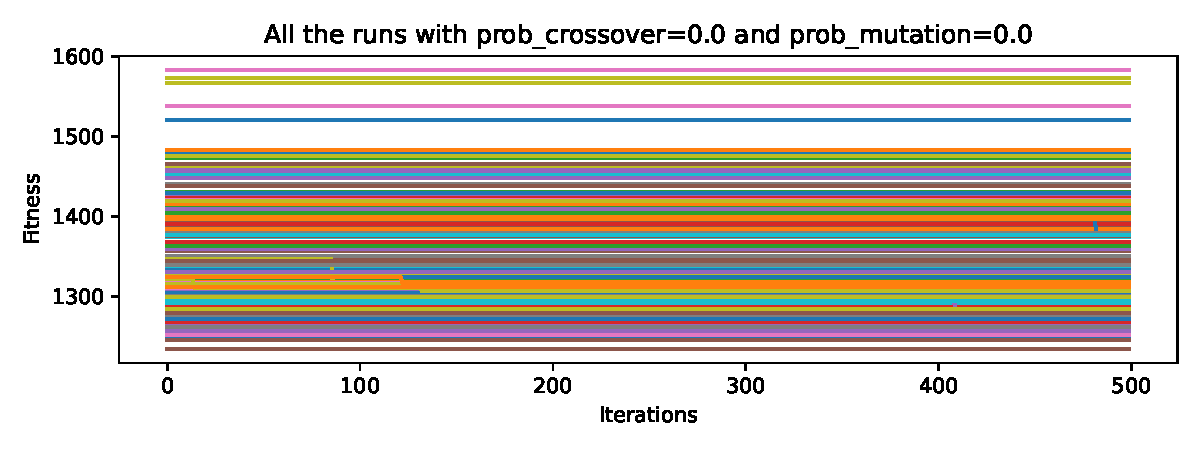
\includegraphics[width=\textwidth]{no_cross_no_mut}
        \caption{When the probability of crossover or mutation is 0 there's no possibility of improvement.}
        \label{fig:prob0}
    \end{figure}

    Depending on the probability values selected for crossover or mutation the speed to achieve an optimal solution
    will be different.
    As it can be seen in Figure~\ref{fig:prob0}, due to not being able to generate new different genomes
    there's no improvement in the fitness metric.

    \begin{figure}[h]
        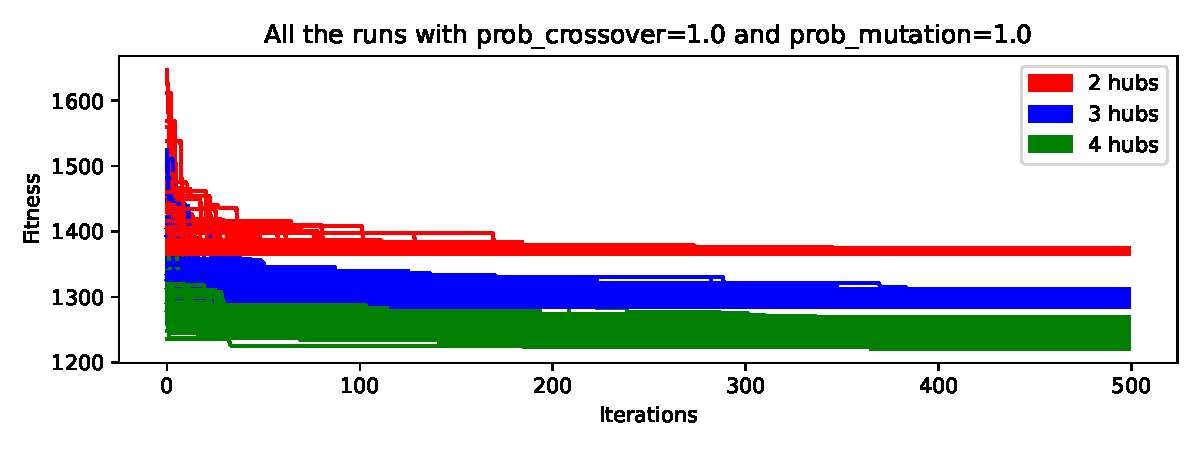
\includegraphics[width=\textwidth]{max_cross_mut}
        \caption{When the probability of crossover or mutation is 1 the variability of final results is big due to
        the big pool of different genomes.}
        \label{fig:prob1}
    \end{figure}

    In the opposite direction of Figure~\ref{fig:prob0}, we can observe in Figure~\ref{fig:prob1} when the crossover
    and mutation probability is at the maximum the variability increases fast so the system is able to achieve a
    bigger variability of results.

    Another interesting observation in Figure~\ref{fig:prob1} is the different fitness values that are achieved based on
    the number of hubs.
    As it should be obvious the more hubs you have the more interconnected is the network so the lower the cost is.
    This is why having hubs of zero cost does not make sense because your ideal fitness would be to make a hub in
    every node.

    \begin{figure}[h]
        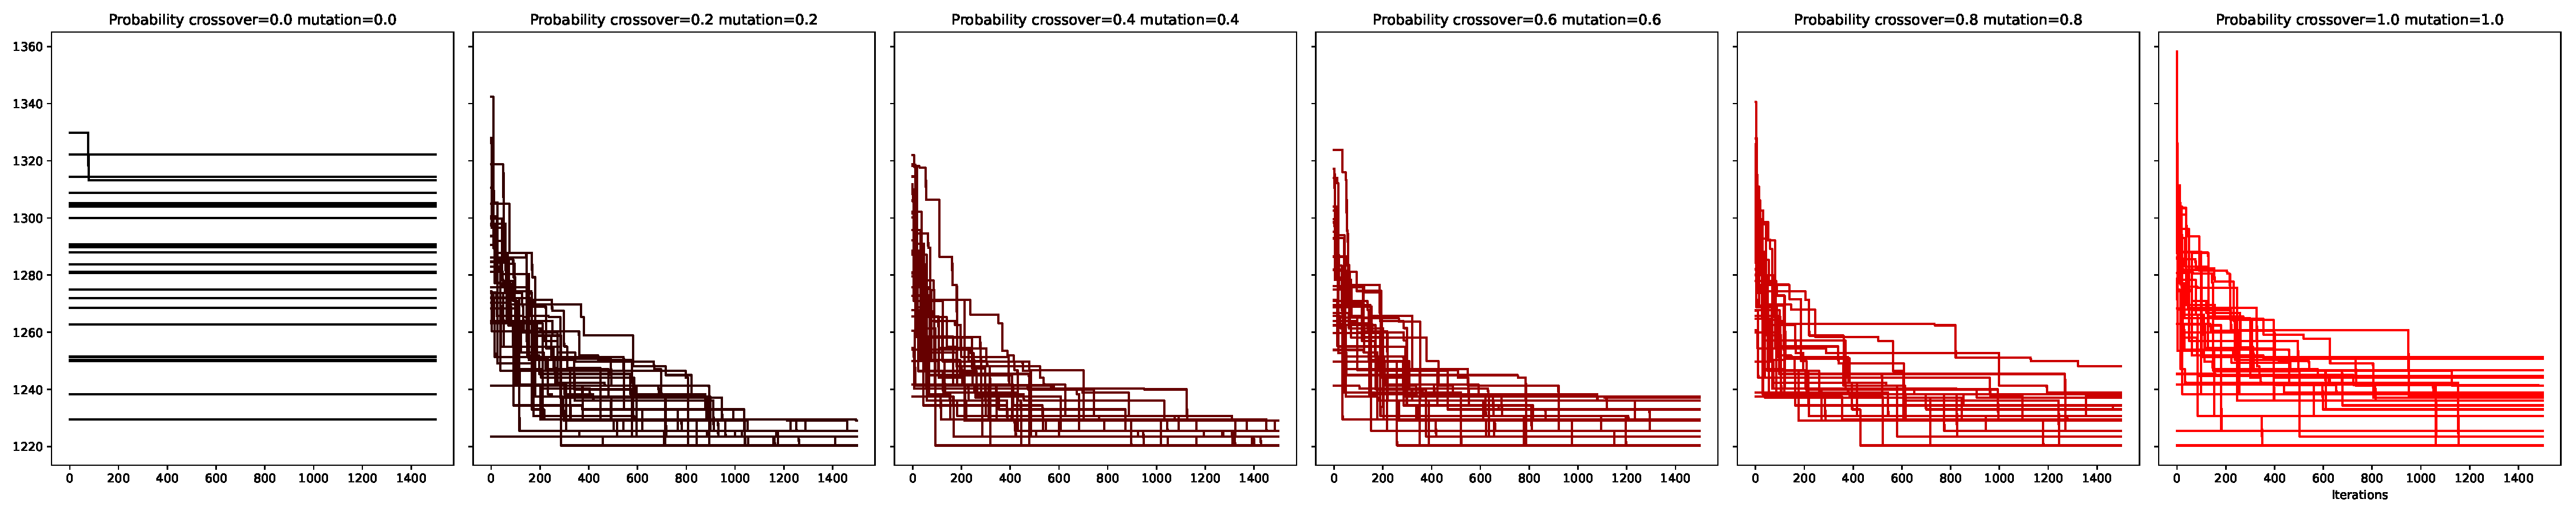
\includegraphics[width=\textwidth]{sweep_values_get_best_fitness}
        \caption{In this figure a sweep from 0 to 1 of the two variables can be seen.}
        \label{fig:sweep_best}
    \end{figure}

    In Figure~\ref{fig:sweep_best} it can be seen that with a bigger value of probability the spread in the final
    results is bigger.
    This is due to the big changes that happen to the genome.
    Every iteration a new individual with a lot of mutations is added, and it has been created from random
    individuals with ver diverse genome keeping the population with a wide spread of genomes.

    \begin{figure}[h]
        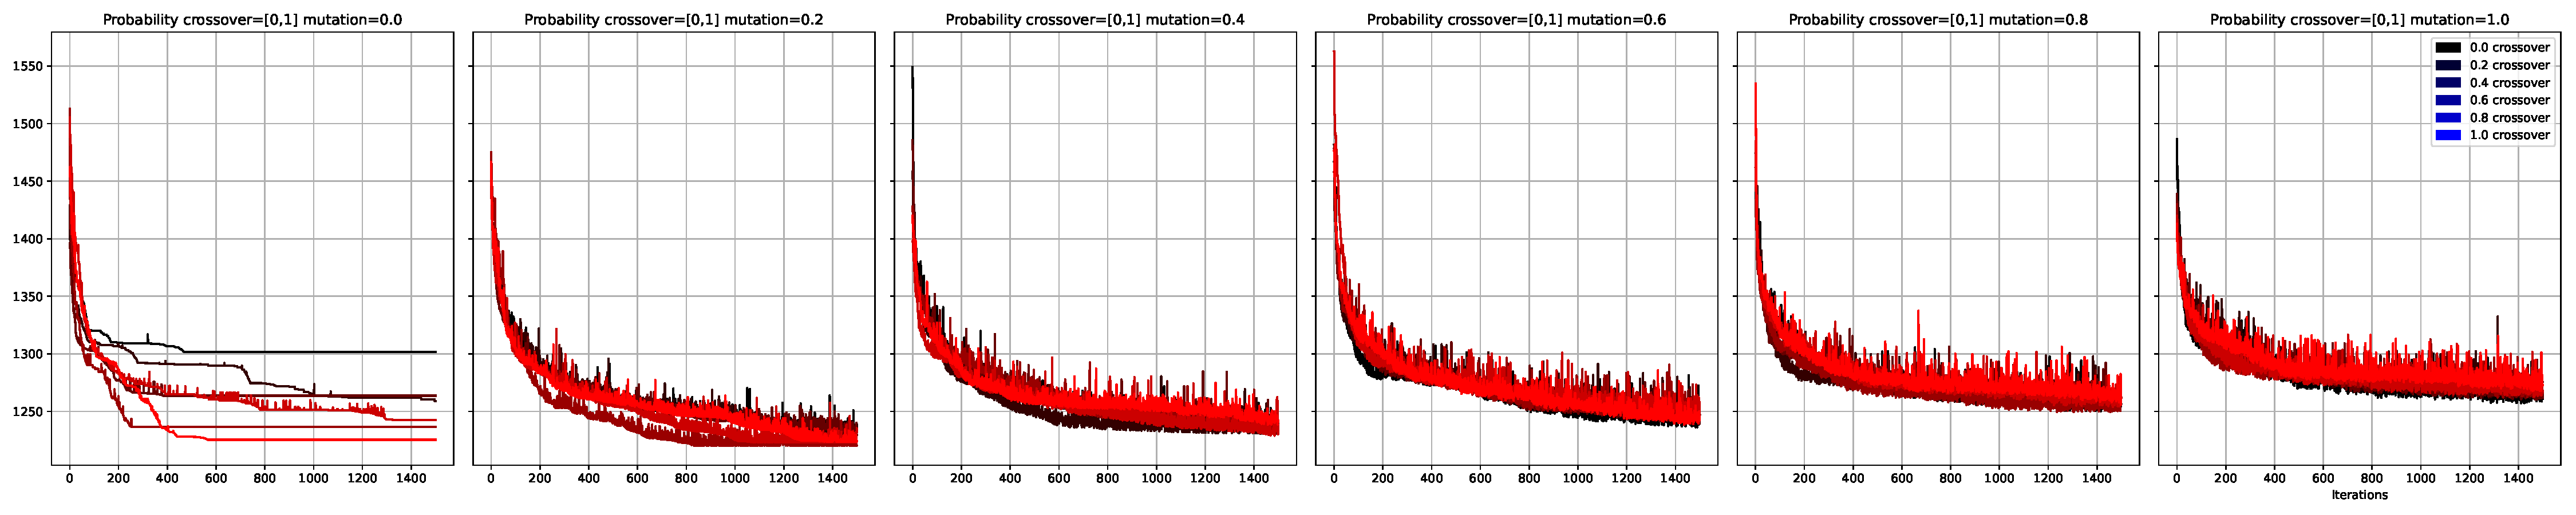
\includegraphics[width=\textwidth]{sweep_values_get_avg_fitness}
        \caption{Similar graph as Figure 3 but in this case the average fitness of the best run for that set of
        values is plotted.
        The intensity of colour indicates a higher probability of crossover.
        Left to right an increased probability
        of mutation.}
        \label{fig:sweep_avg}
    \end{figure}

    In Figure~\ref{fig:sweep_avg} We can observe that high probability values increase the variability and so it does
    the average value so achieving an optimal result takes much longer.
    Based on the data, a probability of mutation around 0.2 is the best to achieve a fast optimal result.
    Then applying crossover with a probability between 0.4 and 0.6 looks like best setting in this case.





    \newpage

    \subsection{Performance}
    Other than learning and exploration, the implementation in C++ bring an edge of performance to be able to run
    plenty of experiments.
    This implementation has parallel run for the fitness calculation which in the machine used for this work provided
    around x10 more performance.


    \section{Conclusion}



    \newpage
    \bibliographystyle{plain}
    \bibliography{refs}
\end{document}